\documentclass[times]{article}
\usepackage{floatflt}
\usepackage{epsfig}
\usepackage{fancyheadings}

\setlength{\topmargin}{0in}
\setlength{\headheight}{0in}
\setlength{\headsep}{0in}
\setlength{\textheight}{5.25in}

\setlength{\hoffset}{-0.25in}
\setlength{\oddsidemargin}{0in}
\setlength{\textwidth}{7in}

%\setlength{\footskip}{14pt}

\chead{}
\cfoot{}
\setlength{\footrulewidth}{1pt}
\setlength{\headrulewidth}{0pt}

\pagestyle{fancy}
\begin{document}
\begin{center}
{\Huge {\bf Most Valuable Player: A Robot Device Server for Distributed 
            Control}
\vspace{1em}
}

{\huge Brian~P.~Gerkey, Richard~T.~Vaughan, Kasper~St{\o}y,
       Andrew~Howard, Gaurav~S.~Sukhatme, and Maja~J~Matari\'{c}
       University of Southern California}
\end{center}


{\huge
\noindent
$\bullet$ We propose a powerful mechanism for achieving effective data flow 
between sensors, processors, and actuators: {\sl Player}.\\
}

\begin{floatingfigure}{1.95in}
\begin{center}
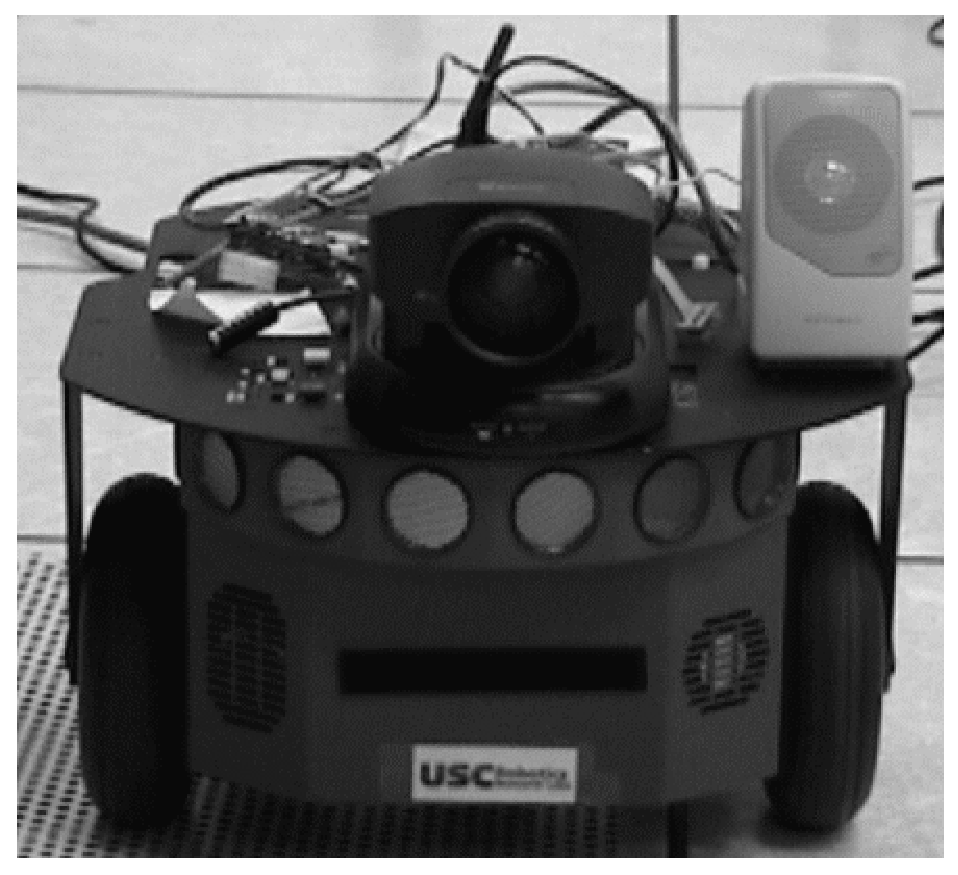
\epsfig{file=pio.eps,width=1.95in}
\end{center}
\end{floatingfigure}

{\huge
\noindent
$\bullet$ Player combines an efficient message protocol with a simple 
device model.\\
}

{\huge
\noindent
$\bullet$ Player is implemented as a TCP socket server 
that provides network access to a collection
of sensors and actuators, often comprising a robot. \\
}

{\huge
\noindent
$\bullet$ The socket abstraction enables platform- and language-independent 
control of these devices.\\ 
}

{\huge
\noindent
$\bullet$ Player is freely available from:
{\Large \verb+http://robotics.usc.edu/player+}.\\
}

\end{document}
